\documentclass{article}

% plain R
% chunk and its name
% fig


\usepackage{Sweave}
\begin{document}
\Sconcordance{concordance:paperVersion_0.tex:paperVersion_0.Rnw:%
1 7 1 1 0 20 1 1 3 2 0 1 1 1 3 1 0 2 1 4 0 1 3 2 1 1 2 1 0 2 1 7 0 1 2 %
1 1 1 2 1 0 1 1 7 0 1 2 1 1 1 2 1 0 1 1 1 3 7 0 1 3 2 1 1 2 1 0 2 1 7 0 %
1 2 2 1 1 2 1 0 1 1 7 0 1 2 1 1 1 2 1 0 1 1 1 3 7 0 1 3 2 1 1 2 1 0 2 1 %
7 0 1 2 2 1 1 2 1 0 1 1 7 0 1 2 1 1 1 2 1 0 1 1 1 3 6 0 1 2 2 1 1 2 1 0 %
2 1 7 0 1 2 2 1 1 2 1 0 1 1 7 0 1 2 2 1 1 2 1 0 1 1 1 3 6 0 1 2 2 1 1 2 %
14 0 1 2 4 1 1 2 1 0 1 2 1 0 1 1 7 0 1 2 5 1 1 3 2 0 1 3 1 0 1 1 9 0 1 %
2 2 1 1 2 1 0 1 1 24 0 1 2 2 1 1 2 1 0 1 1 25 0 1 2 5 1}


LOS INDICES DEL MUNDO


Por: Estrella Delcurso


Introducción

Aqui les presento mi investigacion sobre diversos indices sociales en el mundo. Los indices los conseguí de wikipedia, espero que les gusten mucho.


Exploración Univariada

En esta sección exploro cada índice.




\begin{Schunk}
\begin{Sinput}
> # carga de datos
> filename="indexes.csv"
> dataidx=read.csv(filename, stringsAsFactors = FALSE)
> # previsión:
> level5=c("muy malo","malo","medio","bueno","muy bueno")
> level4=c("muy malo","malo","bueno","muy bueno")
> level3=c("muy malo","medio","muy bueno")
> 
\end{Sinput}
\end{Schunk}


Este es el comportamiento de la democracia en el mundo, veamos primero las frecuencias absolutas:
\begin{Schunk}
\begin{Sinput}
> demoTable=table(dataidx[,5])
> names(demoTable)=level4
> demoTable
\end{Sinput}
\begin{Soutput}
 muy malo      malo     bueno muy bueno 
       60        45        82        19 
\end{Soutput}
\end{Schunk}

Ahora las frecuencias relativas:
\begin{Schunk}
\begin{Sinput}
> demoTableRel=round(prop.table(demoTable)*100,1)
> demoTableRel
\end{Sinput}
\begin{Soutput}
 muy malo      malo     bueno muy bueno 
     29.1      21.8      39.8       9.2 
\end{Soutput}
\end{Schunk}

Y aquí el plot que representa esta distribución
\begin{Schunk}
\begin{Sinput}
> title='Distribución de la Democracia'
> paleta='red'
> barplot(demoTableRel,main=title,
+         col=paleta,ylim = c(0,100),
+         ylab = "%")
> 
\end{Sinput}
\end{Schunk}
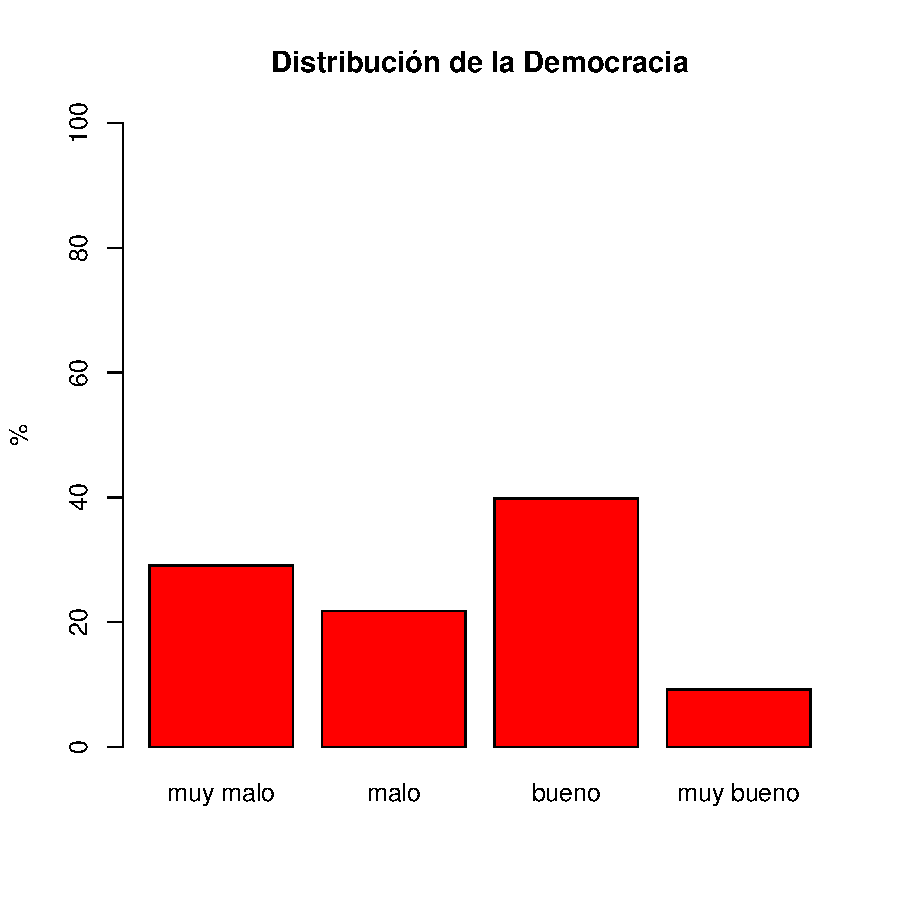
\includegraphics{paperVersion_0-demoTableRelPlot}


La Libertad económica en el mundo en una tabla:
\begin{Schunk}
\begin{Sinput}
> ecoTable=table(dataidx[,3])
> names(ecoTable)=level5
> ecoTable
\end{Sinput}
\begin{Soutput}
 muy malo      malo     medio     bueno muy bueno 
       21        78        74        28         6 
\end{Soutput}
\end{Schunk}


Ahora las frecuencias relativas:
\begin{Schunk}
\begin{Sinput}
> ecoTableRel=round(prop.table(ecoTable)*100,1)
> ecoTableRel
\end{Sinput}
\begin{Soutput}
 muy malo      malo     medio     bueno muy bueno 
     10.1      37.7      35.7      13.5       2.9 
\end{Soutput}
\end{Schunk}

Y aquí el plot que representa esta distribución
\begin{Schunk}
\begin{Sinput}
> title='Distribución de la Libertad Económica'
> paleta='red'
> barplot(ecoTableRel,main=title,
+         col=paleta,ylim = c(0,100),
+         ylab = "%")
> 
\end{Sinput}
\end{Schunk}
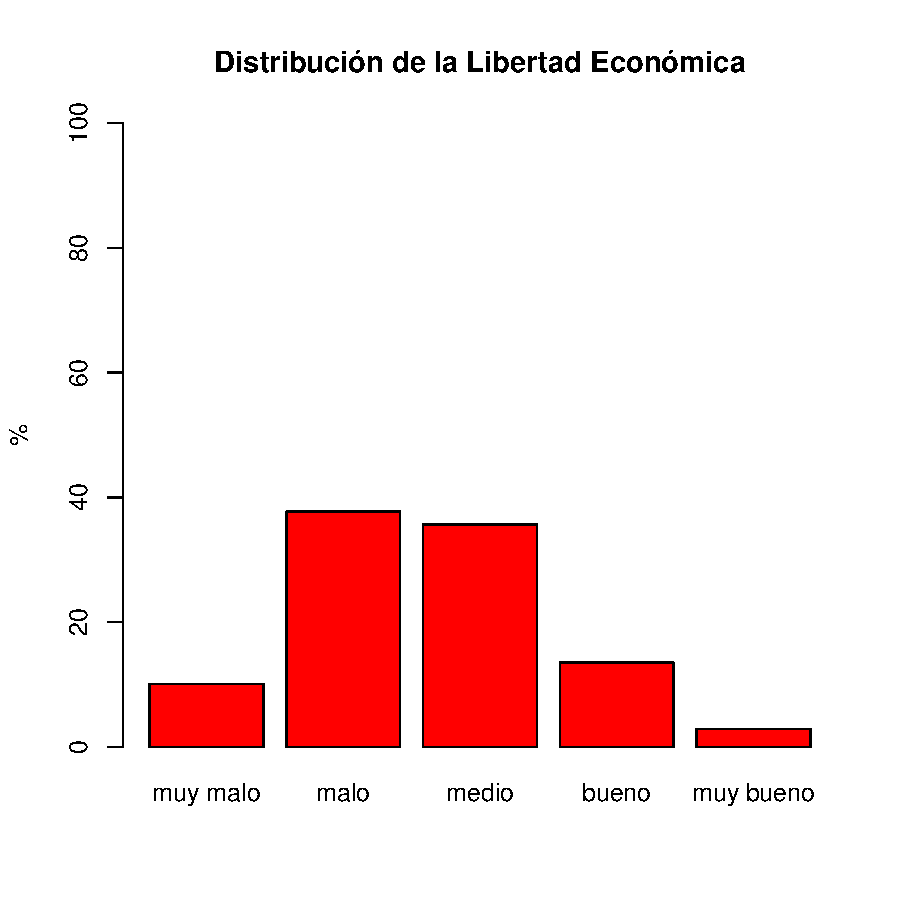
\includegraphics{paperVersion_0-ecoTableRelPlot}


La Libertad general en el mundo en una tabla:
\begin{Schunk}
\begin{Sinput}
> worldTable=table(dataidx[,2])
> names(worldTable)=level3
> worldTable
\end{Sinput}
\begin{Soutput}
 muy malo     medio muy bueno 
       55        62        89 
\end{Soutput}
\end{Schunk}


Ahora las frecuencias relativas:
\begin{Schunk}
\begin{Sinput}
> worldTableRel=round(prop.table(worldTable)*100,1)
> worldTableRel
\end{Sinput}
\begin{Soutput}
 muy malo     medio muy bueno 
     26.7      30.1      43.2 
\end{Soutput}
\end{Schunk}

Y aquí el plot que representa esta distribución
\begin{Schunk}
\begin{Sinput}
> title='Distribución de la Libertad en el Mundo'
> paleta='red'
> barplot(worldTableRel,main=title,
+         col=paleta,ylim = c(0,100),
+         ylab = "%")
\end{Sinput}
\end{Schunk}
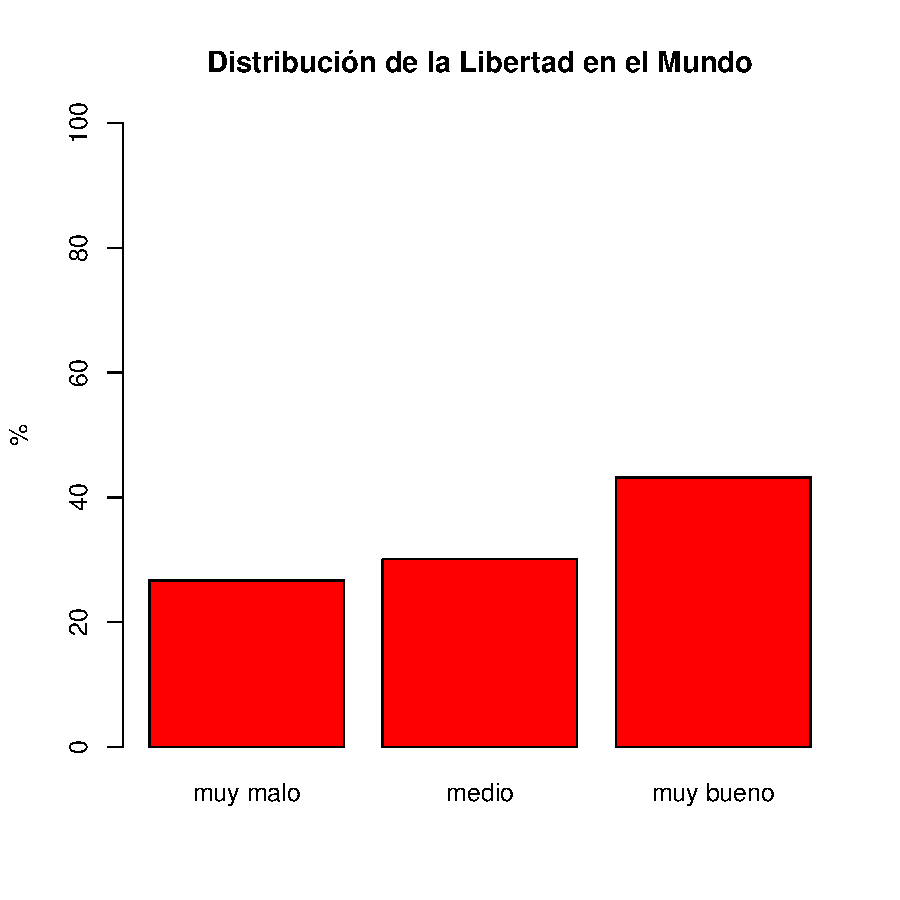
\includegraphics{paperVersion_0-worldTableRelPlot}


La Libertad de prensa en el mundo en una tabla:
\begin{Schunk}
\begin{Sinput}
> pressTable=table(dataidx[,4])
> names(pressTable)=level5
> pressTable
\end{Sinput}
\begin{Soutput}
 muy malo      malo     medio     bueno muy bueno 
       22        53        66        48        17 
\end{Soutput}
\end{Schunk}


Ahora las frecuencias relativas:
\begin{Schunk}
\begin{Sinput}
> pressTableRel=round(prop.table(pressTable)*100,1)
> pressTableRel
\end{Sinput}
\begin{Soutput}
 muy malo      malo     medio     bueno muy bueno 
     10.7      25.7      32.0      23.3       8.3 
\end{Soutput}
\end{Schunk}


Y aquí el plot que representa esta distribución
\begin{Schunk}
\begin{Sinput}
> title='Distribución de la Libertad de Prensa'
> paleta='red'
> barplot(pressTableRel,main=title,
+         col=paleta,ylim = c(0,100),
+         ylab = "%")
\end{Sinput}
\end{Schunk}
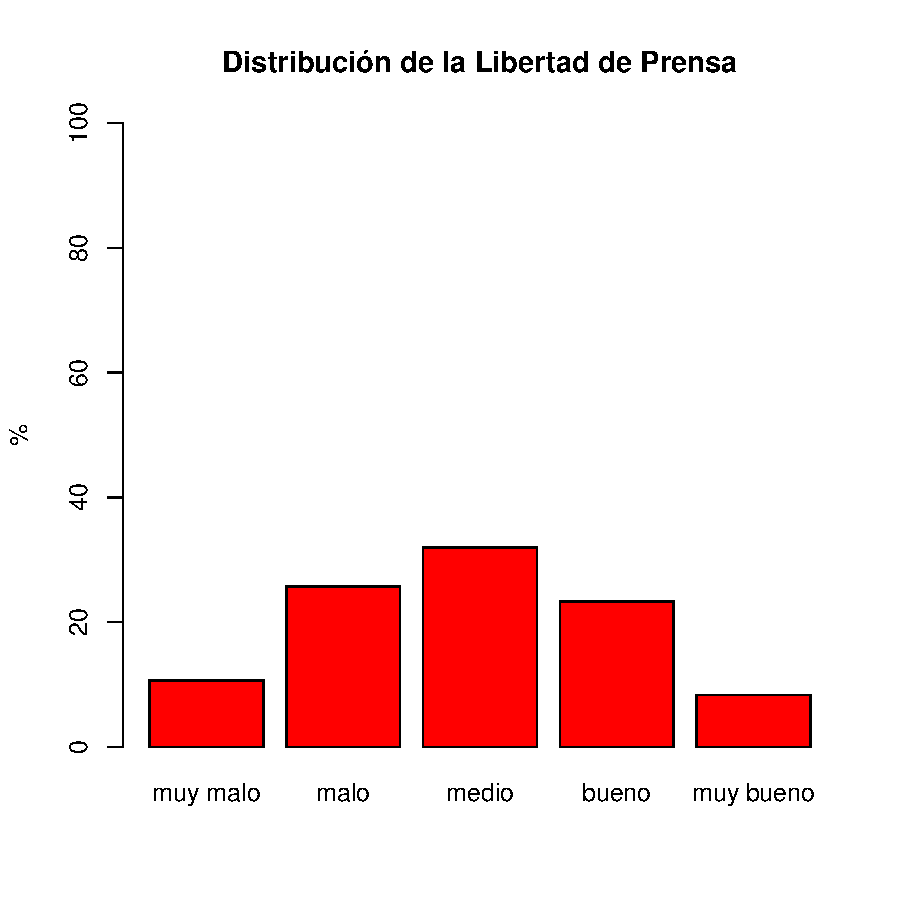
\includegraphics{paperVersion_0-pressTableRelPlot}


Podemos mostrar los estadísticos de cada variable:
\begin{Schunk}
\begin{Sinput}
> summary(dataidx[,-1])
\end{Sinput}
\begin{Soutput}
  WorldFreedom  EconomicFreedom  PressFreedom     Democracy    
 Min.   :1.00   Min.   :1.000   Min.   :1.000   Min.   :1.000  
 1st Qu.:1.00   1st Qu.:2.000   1st Qu.:2.000   1st Qu.:1.000  
 Median :3.00   Median :3.000   Median :3.000   Median :2.000  
 Mean   :3.33   Mean   :2.614   Mean   :2.927   Mean   :2.782  
 3rd Qu.:5.00   3rd Qu.:3.000   3rd Qu.:4.000   3rd Qu.:4.000  
 Max.   :5.00   Max.   :5.000   Max.   :5.000   Max.   :5.000  
 NA's   :1                      NA's   :1       NA's   :1      
\end{Soutput}
\end{Schunk}


Exploración Bivariada

En este trabajo estamos interesados en el impacto de los otros indices en el nivel de Democracia. Veamos las relaciones bivariadas que tiene esta variable con todas las demás:
\begin{Schunk}
\begin{Sinput}
> explanans=names(dataidx)[c(2:4)]
> corrDem=cor(dataidx[,5],dataidx[,explanans],
+     use = "na.or.complete")
> corrDem
\end{Sinput}
\begin{Soutput}
     WorldFreedom EconomicFreedom PressFreedom
[1,]    0.8962136       0.5865487    0.7710711
\end{Soutput}
\end{Schunk}




Veamos la correlación entre las variables independientes:

\begin{Schunk}
\begin{Sinput}
> corrTable=round(cor(dataidx[explanans],
+                use = "na.or.complete"),2)
> # Hide upper triangle
> corrTable[upper.tri(corrTable)]<-""
> as.data.frame(corrTable)
\end{Sinput}
\begin{Soutput}
                WorldFreedom EconomicFreedom PressFreedom
WorldFreedom               1                             
EconomicFreedom         0.49               1             
PressFreedom            0.83            0.53            1
\end{Soutput}
\end{Schunk}


Finalmente, vemos los modelos propuestos. Primero sin la libertad mundial como independiente:
\begin{Schunk}
\begin{Sinput}
> LinRegA = lm(Democracy ~ ., data = dataidx[,c(3:5)])
> summary(LinRegA)
\end{Sinput}
\begin{Soutput}
Call:
lm(formula = Democracy ~ ., data = dataidx[, c(3:5)])

Residuals:
     Min       1Q   Median       3Q      Max 
-1.99066 -0.61319  0.05363  0.43110  2.22022 

Coefficients:
                Estimate Std. Error t value Pr(>|t|)    
(Intercept)     -0.64197    0.19912  -3.224  0.00147 ** 
EconomicFreedom  0.37747    0.07736   4.879 2.15e-06 ***
PressFreedom     0.83341    0.06509  12.804  < 2e-16 ***
---
Signif. codes:  0 ‘***’ 0.001 ‘**’ 0.01 ‘*’ 0.05 ‘.’ 0.1 ‘ ’ 1

Residual standard error: 0.88 on 203 degrees of freedom
  (1 observation deleted due to missingness)
Multiple R-squared:  0.6371,	Adjusted R-squared:  0.6335 
F-statistic: 178.2 on 2 and 203 DF,  p-value: < 2.2e-16
\end{Soutput}
\end{Schunk}

Luego con la libertad mundial

\begin{Schunk}
\begin{Sinput}
> LinRegB = lm(Democracy ~ ., data = dataidx[,c(2:5)])
> summary(LinRegB)
\end{Sinput}
\begin{Soutput}
Call:
lm(formula = Democracy ~ ., data = dataidx[, c(2:5)])

Residuals:
     Min       1Q   Median       3Q      Max 
-1.78162 -0.36268 -0.07215  0.30011  1.91679 

Coefficients:
                Estimate Std. Error t value Pr(>|t|)    
(Intercept)     -0.35412    0.13782  -2.569   0.0109 *  
WorldFreedom     0.70394    0.04642  15.164  < 2e-16 ***
EconomicFreedom  0.29053    0.05335   5.446 1.49e-07 ***
PressFreedom     0.01166    0.07020   0.166   0.8683    
---
Signif. codes:  0 ‘***’ 0.001 ‘**’ 0.01 ‘*’ 0.05 ‘.’ 0.1 ‘ ’ 1

Residual standard error: 0.6033 on 202 degrees of freedom
  (1 observation deleted due to missingness)
Multiple R-squared:  0.8303,	Adjusted R-squared:  0.8278 
F-statistic: 329.4 on 3 and 202 DF,  p-value: < 2.2e-16
\end{Soutput}
\end{Schunk}





\end{document}
